% Options for packages loaded elsewhere
\PassOptionsToPackage{unicode}{hyperref}
\PassOptionsToPackage{hyphens}{url}
%
\documentclass[
  17pt,
  a4paper]{extarticle}
\title{Analysis 1B --- Week 11}
\author{Christian Jones: University of Bath}
\date{May 2023}

\usepackage{amsmath,amssymb}
\usepackage{lmodern}
\usepackage{iftex}
\ifPDFTeX
  \usepackage[T1]{fontenc}
  \usepackage[utf8]{inputenc}
  \usepackage{textcomp} % provide euro and other symbols
\else % if luatex or xetex
  \usepackage{unicode-math}
  \defaultfontfeatures{Scale=MatchLowercase}
  \defaultfontfeatures[\rmfamily]{Ligatures=TeX,Scale=1}
\fi
% Use upquote if available, for straight quotes in verbatim environments
\IfFileExists{upquote.sty}{\usepackage{upquote}}{}
\IfFileExists{microtype.sty}{% use microtype if available
  \usepackage[]{microtype}
  \UseMicrotypeSet[protrusion]{basicmath} % disable protrusion for tt fonts
}{}
\makeatletter
\@ifundefined{KOMAClassName}{% if non-KOMA class
  \IfFileExists{parskip.sty}{%
    \usepackage{parskip}
  }{% else
    \setlength{\parindent}{0pt}
    \setlength{\parskip}{6pt plus 2pt minus 1pt}}
}{% if KOMA class
  \KOMAoptions{parskip=half}}
\makeatother
\usepackage{xcolor}
\IfFileExists{xurl.sty}{\usepackage{xurl}}{} % add URL line breaks if available
\IfFileExists{bookmark.sty}{\usepackage{bookmark}}{\usepackage{hyperref}}
\hypersetup{
  pdftitle={Analysis 1B --- Week 11},
  pdfauthor={Christian Jones: University of Bath},
  hidelinks,
  pdfcreator={LaTeX via pandoc}}
\urlstyle{same} % disable monospaced font for URLs
\usepackage[margin=2.5cm]{geometry}
\usepackage{longtable,booktabs,array}
\usepackage{calc} % for calculating minipage widths
% Correct order of tables after \paragraph or \subparagraph
\usepackage{etoolbox}
\makeatletter
\patchcmd\longtable{\par}{\if@noskipsec\mbox{}\fi\par}{}{}
\makeatother
% Allow footnotes in longtable head/foot
\IfFileExists{footnotehyper.sty}{\usepackage{footnotehyper}}{\usepackage{footnote}}
\makesavenoteenv{longtable}
\usepackage{graphicx}
\makeatletter
\def\maxwidth{\ifdim\Gin@nat@width>\linewidth\linewidth\else\Gin@nat@width\fi}
\def\maxheight{\ifdim\Gin@nat@height>\textheight\textheight\else\Gin@nat@height\fi}
\makeatother
% Scale images if necessary, so that they will not overflow the page
% margins by default, and it is still possible to overwrite the defaults
% using explicit options in \includegraphics[width, height, ...]{}
\setkeys{Gin}{width=\maxwidth,height=\maxheight,keepaspectratio}
% Set default figure placement to htbp
\makeatletter
\def\fps@figure{htbp}
\makeatother
\setlength{\emergencystretch}{3em} % prevent overfull lines
\providecommand{\tightlist}{%
  \setlength{\itemsep}{0pt}\setlength{\parskip}{0pt}}
\setcounter{secnumdepth}{5}
\newcommand{\BOO}{BOO}
\usepackage {hyperref}
\hypersetup {colorlinks = true, linkcolor = blue, urlcolor = blue}
\usepackage{float}
\ifLuaTeX
  \usepackage{selnolig}  % disable illegal ligatures
\fi

\usepackage{amsthm}
\theoremstyle{plain}
\newtheorem*{theorem*}{Theorem}\newtheorem{theorem}{Theorem}[section]
\theoremstyle{definition}
\newtheorem*{definition*}{Definition}\newtheorem{definition}{Definition}[section]
\theoremstyle{plain}
\newtheorem*{proposition*}{Proposition}\newtheorem{proposition}[theorem]{Proposition}
\newtheorem*{Definitions*}{Definitions}\newtheorem{Definitions}[definition]{Definitions}
\theoremstyle{plain}
\newtheorem*{lemma*}{Lemma}\newtheorem{lemma}{Lemma}[section]
\theoremstyle{plain}
\newtheorem*{corollary*}{Corollary}\newtheorem{corollary}{Corollary}[section]
\theoremstyle{plain}
\newtheorem*{conjecture*}{Conjecture}\newtheorem{conjecture}{Conjecture}[section]
\theoremstyle{definition}
\newtheorem*{example*}{Example}\newtheorem{example}{Example}[section]
\theoremstyle{definition}
\newtheorem*{exercise*}{Exercise}\newtheorem{exercise}{Exercise}[section]
\newtheorem*{Non-theorem*}{Non-theorem}\newtheorem{Non-theorem}{Non-theorem}[section]
\newtheorem*{Question*}{Question}\newtheorem{Question}{Question}[section]
\newtheorem*{Thought*}{Thought}\newtheorem{Thought}{Thought}[section]
\theoremstyle{remark}
\newtheorem*{remark*}{Remark}
\newtheorem*{solution*}{Solution}
\newtheorem*{Example*}{Example}
\theoremstyle{remark}
\newtheorem*{Proof*}{Proof}
\newtheorem*{Examples*}{Examples}
\let\BeginKnitrBlock\begin \let\EndKnitrBlock\end


%\usepackage[english,shorthands=off]{babel}
\usepackage{etoolbox}
\usepackage{spverbatim}
\makeatletter
\@ifpackageloaded{float}{}{\usepackage{float}}
\@ifpackageloaded{adjustbox}{}{\usepackage[Export]{adjustbox}}
\makeatother
\floatplacement{figure}{H}
\newcommand{\scalefactor}{1.7}
\adjustboxset*{min width=\scalefactor\width,max width=\linewidth}
\renewcommand{\familydefault}{phv}
\fontfamily{phv}\selectfont
\renewcommand{\em}{\bf}\renewcommand{\textit}{\textbf}\renewcommand{\emph}{\textbf}\renewcommand{\it}{\bf}\renewcommand{\itshape}{\bf}
\setlength{\parindent}{0.0pt}
\setlength{\parskip}{1.0\baselineskip}
\renewcommand{\baselinestretch}{1.5}\selectfont
\setlength{\mathsurround}{0.2em}
\setlength{\arraycolsep}{0.5cm}\renewcommand{\arraystretch}{1.5}
\addtolength{\jot}{\baselineskip}
\renewcommand{\;}{\,}
\sloppy
\allowdisplaybreaks
\usepackage{amsthm}
\newtheoremstyle{plain}{20pt}{3pt}{}{}{\bfseries}{.\newline\nobreak}{1.0em\nobreak}{}
\newtheoremstyle{definition}{20pt}{3pt}{}{}{\bfseries}{.\newline\nobreak}{1.0em\nobreak}{}
\newtheoremstyle{remark}{20pt}{3pt}{}{}{\bfseries}{.\newline\nobreak}{1.0em\nobreak}{}
\csundef{Proof}
\csundef{endProof}
\newenvironment{Proof}
  {\noindent{\bf Proof.}\hspace*{1em}}% Begin
  {\qed\par}% End
%% When redefining an environment it is vital that it has 
%% the same number of arguments as the original
\renewenvironment{proof}[1][\proofname]
  {\trivlist\item\relax\noindent{\bf {#1}.}\hspace*{1em}}% Begin
  {\qed\endtrivlist}% End

\begin{document}
\maketitle

{
\setcounter{tocdepth}{2}
\tableofcontents
}
\newpage
\pagenumbering{arabic}

\hypertarget{introduction}{%
\section*{Introduction}\label{introduction}}
\addcontentsline{toc}{section}{Introduction}

Here is the material to accompany Week 11 of the Analysis 1B course. Alternative formats can be downloaded by clicking the download icon at the top of the page. Please send any comments or corrections to \href{mailto:caj50@bath.ac.uk}{Christian Jones (caj50)}. To return to the homepage, click \href{http://caj50.github.io/tutoring.html}{here}.

\hypertarget{lecture-recap}{%
\section{Lecture Recap}\label{lecture-recap}}

There's no tutorial this week due to the May Day bank holiday. However, there's still a bit of the course to summarise (including the fundamental theorem of calculus). So here, you'll find some material that would have been covered if everything was running as normal.

\hypertarget{some-integral-theorems}{%
\subsection{Some Integral Theorems}\label{some-integral-theorems}}

We begin with two theorems, which basically say that integrals behave as you'd expect them to.

\BeginKnitrBlock{theorem}[Additivity of the Integral]
{\label{thm:thm1} }Let \(a<b\) and let \(f:[a,b] \to \mathbb{R}\) be bounded. For any \(c \in (a,b)\), \(f\) is integrable on \([a,b]\) if and only if \(f\) is integrable on \([a,c]\) and \([c,b].\) In this case \[\int_a^b f = \int_a^c f + \int_c^b f.\]
\EndKnitrBlock{theorem}

We can see this theorem in action below in Figure \ref{fig:additivity}.

\begin{figure}

{\centering 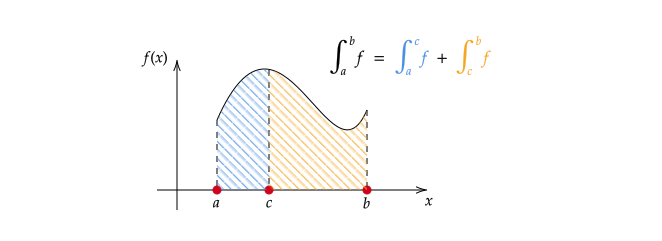
\includegraphics[width=\Width,height=\Height]{Additivity} 

}

\caption{The integral being additive means that to integrate a function $f$ on a domain $[a,b]$, we can just sum up the integrals of $f$ on some smaller domains. This is especially useful for functions defined piecewise.}\label{fig:additivity}
\end{figure}

\BeginKnitrBlock{theorem}[Linearity of the Integral]
{\label{thm:thm2} }Let \(a<b\), \(\lambda \in \mathbb{R}\) and let \(f,g:[a,b] \to \mathbb{R}\) be integrable. Then

\begin{enumerate}
\def\labelenumi{\arabic{enumi})}
\tightlist
\item
  \(f+g\) is integrable, with \[\int_a^b f+g = \int_a^b f + \int_a^b g,\]
\item
  \(\lambda f\) is integrable, with \[\int_a^b \lambda f = \lambda \int_a^b f.\]
\end{enumerate}
\EndKnitrBlock{theorem}

Now is the time to bring some algebra into the mix. Since the zero function \(0:[a,b] \to \mathbb{R}\) given by \(0(x) = 0\) is integrable, this means that the set of integrable functions on \([a,b]\) is a vector subspace of the set of bounded functions on \([a,b]\).

\hypertarget{useful-results-about-sup-and-inf.}{%
\subsubsection{\texorpdfstring{Useful Results about \(\sup\) and \(\inf\).}{Useful Results about \textbackslash sup and \textbackslash inf.}}\label{useful-results-about-sup-and-inf.}}

To prove the above two theorems, we need to know a bit about how the bounds of a sum of two bounded functions behave. The following results tell us exactly what we want!

\BeginKnitrBlock{proposition}
{\label{prp:prop1} }For \(I \subseteq \mathbb{R}\) non-empty, \(\lambda \in \mathbb{R}\) and \(f,g:I \to \mathbb{R}\) bounded. Then:

\begin{itemize}
\tightlist
\item
  \(f+g\) is bounded, with \[\sup_{I}(f + g) \leq \sup_{I}f + \sup_{I}g, \quad \inf_{I}(f + g) \geq \inf_{I}f + \inf_{I}g\]
\item
  If \(\lambda \geq 0\): \[\sup_{I}(\lambda f) = \lambda\sup_{I}f, \;\; \inf_{I}(\lambda f) = \lambda\inf_{I}f,\]
\item
  If \(\lambda < 0\): \[\sup_{I}(\lambda f) = \lambda\inf_{I}f, \;\; \inf_{I}(\lambda f) = \lambda\sup_{I}f,\]
\end{itemize}
\EndKnitrBlock{proposition}

\hypertarget{some-other-useful-facts}{%
\subsubsection{Some Other Useful Facts}\label{some-other-useful-facts}}

Using everything we've learned so far, we can state a few more facts about integrals!

\BeginKnitrBlock{proposition}
{\label{prp:prop2} }If \(a<b\) and \(f,g:[a,b] \to \mathbb{R}\) are integrable, then:

\begin{enumerate}
\def\labelenumi{\arabic{enumi})}
\tightlist
\item
  \(\int_a^a f = 0\) (This is by definition!)
\item
  \(\int_b^a f := -\int_a^b f\) (This is also by definition!)
\item
  The function \(f \cdot g\) is integrable (recall \((f\cdot g)(x) = f(x)g(x)\))
\item
  \(\lvert f \rvert\) is integrable, with \[\left\lvert\int_a^b f \right\rvert \leq \int_a^b \lvert f \rvert.\]
\end{enumerate}
\EndKnitrBlock{proposition}

It's worth mentioning here that point 4 above is actually an analogue of the triangle inequality for integrals!

\hypertarget{the-fundamental-theorems-of-calculus}{%
\subsection{The Fundamental Theorem(s) of Calculus}\label{the-fundamental-theorems-of-calculus}}

We've finally made it to the biggest theorems of the course, and this ties in everything done in the last 11 weeks! Despite usually being called \emph{the} fundamental theorem of calculus (FTC), it actually encompasses two statements, which is why we state them separately below:

\BeginKnitrBlock{theorem}[Fundamental Theorem of Calculus I]
{\label{thm:thm3} }Let \(a<b\) and \(I \subseteq \mathbb{R}\) be an open interval containing \([a,b]\). Let \(F:I \to \mathbb{R}\) be differentiable on \(I\), and let \(f:[a,b] \to \mathbb{R}\) be such that

\begin{itemize}
\tightlist
\item
  \(f(x) = F'(x) \;\; \forall x \in [a,b]\),\footnote{This is the definition of \(F\) being a \emph{primitive} for \(f\).}
\item
  \(f\) is integrable on \([a,b]\).
\end{itemize}

Then \[\int_a^b f  = F(b) - F(a).\]
\EndKnitrBlock{theorem}

\BeginKnitrBlock{theorem}[Fundamental Theorem of Calculus II]
{\label{thm:thm4} }Let \(f:[a,b] \to \mathbb{R}\) be integrable, and define \(F;[a,b] \to \mathbb{R}\) via \[F(x) = \int_a^x f.\] Then

\begin{itemize}
\tightlist
\item
  \(F\) is continuous on \([a,b],\) and
\item
  If \(f\) is continuous at \(c \in (a,b)\), then \(F\) is differentiable at \(c \in (a,b)\) with \(F'(c) = f(c).\)
\end{itemize}
\EndKnitrBlock{theorem}

So, why should we like these theorems so much? The first theorem makes finding integrals much easier, as derivatives are (generally) nicer to deal with than Riemann sums! The second theorem here gives you \emph{existence} of a primitive for \(f\), which you can apply the first theorem to!

As a warning, if in Theorem \ref{thm:thm4} \(f\) is \textbf{not} continuous at \(c \in (a,b)\), \(F\) may still be differentiable at \(c\)! See Problem Sheet 11, Tutorial Question 1 for more details.

\hypertarget{integration-techniques}{%
\subsection{Integration Techniques}\label{integration-techniques}}

To finish the lecture recap, it would be handy to have some theorems which back up some standard integration techniques. Turns out that we do! The first of these (in a fashion) `undoes' the differential product rule.

\BeginKnitrBlock{theorem}[Integration By Parts]
{\label{thm:thm5} }Let \(f,g:[a,b] \to \mathbb{R}\) be continuous. Suppose that \(F,G:[a,b] \to \mathbb{R}\) are continuous on \([a,b]\) and differentiable on \((a,b)\) with \(F'(x) = f(x)\) and \(G'(x) = g(x)\;\; \forall x \in (a,b).\) Then \[\int_a^b fG = F(b)G(b) - F(a)G(a) - \int_a^b Fg.\]
\EndKnitrBlock{theorem}

And finally, the second of these can be seen as a way of `undoing' the differential chain rule.

\BeginKnitrBlock{theorem}[Integration By Substitution]
{\label{thm:thm6} }Let \(I \subseteq \mathbb{R}\) be a closed interval and let \(f:I \to \mathbb{R}\) be continuous on \(I\). Also, let \(J \subseteq \mathbb{R}\) be an open interval, and let \(u: J \to I\) be continuously differentiable\footnote{This means that \(u\) is differentiable on \(J\), and that the derivative \(u'\) is continuous on \(J\). For interest, the set of all continuously differentiable functions from a set \(J\) is denoted by \(C^{1}(J)\).}. Then, for \(a,b \in J\), \[\int_a^b (f \circ u) u' = \int_{u(a)}^{u(b)} f.\]
\EndKnitrBlock{theorem}

\end{document}
